\section[Some Special Functions]{\hyperlink{toc}{Some Special Functions}}

\subsection{Power Series, Revisited}
Recall our definition of power series (Definition \ref{def:3.38}), functions of the form:
\begin{align*}
    f(x) = \sum_{n=0}^\infty c_n x^n.
\end{align*}
Also recall the radius of convergence (Theorem \ref{thm:3.39}) of such power series, defined as:
\begin{align*}
    R = \frac{1}{\limsup_{n \rightarrow \infty}\sqrt[n]{\abs{c_n}}}.
\end{align*}
Note that if $\limsup_{n \rightarrow \infty}\sqrt[n]{\abs{c_n}} = \infty$, then $R = 0$, and if $\limsup_{n \rightarrow \infty}\sqrt[n]{\abs{c_n}} = 0$, then $R = \infty$. The series converges absolutely for $\abs{x} < R$ and diverges for $\abs{x} > R$.

\begin{figure}[htbp]
    \centering
    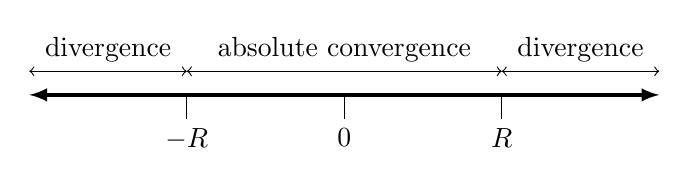
\begin{tikzpicture}[scale=2]
        \draw[latex-latex, very thick] (-2, 0) -- (2, 0);
        \draw[] (0, 0) -- (0, -0.15);
        \draw[] (1, 0) -- (1, -0.15);
        \draw[] (-1, 0) -- (-1, -0.15);
        \node[below] at (0, -0.15) {$0$};
        \node[below] at (1, -0.15) {$R$};
        \node[below] at (-1, -0.15) {$-R$};
        \draw[<->] (1, 0.15) -- (-1, 0.15);
        \draw[<->] (1, 0.15) -- (2, 0.15);
        \draw[<->] (-1, 0.15) -- (-2, 0.15);
        \node[above] at (0, 0.15) {absolute convergence};
        \node[above] at (1.5, 0.15) {divergence};
        \node[above] at (-1.5, 0.15) {divergence};
    \end{tikzpicture}
    
    \caption{Visualization of the radius of convergence for $f(x) = \sum_{n=0}^\infty c_nx^n$, $x \in \RR$.}
    \label{fig49}
\end{figure}

\begin{theorem}{}{8.1}
    If $\sum_{n=0}^\infty c_nx^n$ converges for $\abs{x} < R$, let $f(x) = \sum_{n=0}^\infty c_n x^n$ for $\abs{x} < R$. Then, the series converges uniformly on $[-R + \e, R - \e]$ for any $\e > 0$, $f$ is differentiable (and hence continuous) on $(-R, R)$ and $f'(x) = \sum_{n=0}^\infty nc_nx^{n-1}$. 
\end{theorem}

\begin{nproof}
    We first show the uniform convergence on $[-R + \e, R - \e]$. For $\abs{x} \leq R - \e$, we have that $\abs{c_nx^n} \leq \abs{x_n}(R - \e)^n$. Since $\sum_n \abs{c_n}(R - \e)^n < \infty$ (by the assumed absolute convergence on $(-R, R)$), we have that $\sum_n c_nx^n$ converges uniformly in $\abs{x} \leq R - \e$ by the M-test (Theorem \ref{thm:7.10}).

    We next prove the claim about the differentiability/derivative of $f$. The radius of convergence of $\sum_n nc_n x^{n-1}$ is:
    \begin{align*}
        \frac{1}{\limsup_{n \rightarrow \infty}\sqrt[n]{\abs{nc_n}}} = \frac{1}{\limsup_{n \rightarrow \infty}\sqrt[n]{\abs{c_n}}} = R
    \end{align*}
    so since $f$ converges in $(-R, R)$, so does $\sum_n nc_nx^{n-1}$. Now, let $s_n(x) = \sum_{m=0}^n c_mx^m$. Then, by the linearity of the derivative we have that $s_n'(x) = \sum_{m=1}^n mc_mx^{m-1}$. By the first part of the proof, we have that $s_n'(x) \rightarrow \sum_{m=1}^\infty mc_mx^{m-1}$ uniformly on $[-R + \e, R - \e]$. Since $s_n(x) \rightarrow f(x)$ uniformly, by Theorem \ref{thm:7.17}, we have that $f'$ exists on $[-R +\e, R - \e]$ and $f'(x) = \sum_{m=1}^\infty mc_mx^{m-1}$. Since $\e$ is arbitrary, $f'$ exists and is equal to $\sum_{m=1}^\infty mc_mx^{m-1}$ for all $x \in (-R, R)$. \qed 
\end{nproof}
\noindent As a remark, note that we can (interestingly) prove the differentiability of $f$ on $(-R, R)$ from the uniform convergence on $[-R + \e, R - \e]$.

\begin{ncorollary}{}{}
    If $f(x) = \sum_{n=0}^\infty c_nx^n$ converges for $\abs{x} < R$, then $f^{(k)}(x)$ exists for all $k \in \NN$ and for all $x \in (-R, R)$. It is given by:
    \begin{align*}
        f^{(k)}(x) = \sum_{n=k}^\infty n(n-1)\ldots(n-k+1)c_nx^{n-k} \quad (*)
    \end{align*}
    and consequently, we have that $c_k = \frac{f^{(k)(0)}}{k!}$, so $f(x) = \sum_{n=0}^\infty \frac{f^{(n)}(0)}{n!}x^n$.
\end{ncorollary}
\noindent Compare the above Corollary to Taylor's theorem (Theorem \ref{thm:5.15}). Here, we take our taylor polynomial and extend it to an infinite series (the limit of polynomials). 

\begin{nproof}
    By Theorem \ref{thm:8.1}, we have that $f'(x) = \sum_{n=1}^\infty nc_nx^{n-1}$ and $f''(x) = \sum_{n=2}^\infty n(n-1)c_nx^{n-2}$ and so on. Setting $x = 0$ in $(*)$, we have that $f^{(k)}(0) = n(n-1)\ldots 1 c_n = n! c_k$, so $c_n = \frac{f^{(k)}(0)}{n!}$. \qed
\end{nproof}
\noindent Recall the definition of \emph{analytic functions}, which are infinite differentiable and can be represented as sums or series of derivatives evaluated at zero. 

\begin{nexample}{}{}
    As we discussed in Chapter 5, there are infinitely differentiable functions that are not analytic. Let:
    \begin{align*}
        f(x) = \begin{cases}
            \exp(-\frac{1}{x^2}) & x \neq 0
            \\ 0 & x = 0
        \end{cases}
    \end{align*}
    By Theorem \ref{thm:8.1}, $f$ is infinitely differentiable, and $f^{(n)}(0) = 0$ for all $n \in \NN$. But, $f(x) \neq 0$ except at $x = 0$. Hence, $f(x) \neq \sum_{n=0}^\infty \frac{f^{(n)}(0)}{n!}x^n$ except at $x = 0$. This is true despite the fact that the RHS converges to zero for all $x \in \RR$. 
\end{nexample}

\begin{nexample}{}{}
    Bump functions are continuous, infinitely differentiable functions of compact support (it is zero outside of a compact set). For example, 
    \begin{align*}
        f(x) = \begin{cases}
            \exp(-\frac{1}{1-x^2}) & x \in (-1, 1)
            \\ 0 & \abs{x} \geq 1
        \end{cases}
    \end{align*}
    is an example of a bump function. Such functions are very useful in the study of functional analysis and PDEs.
\end{nexample}
\begin{figure}[htbp]
    \centering
    \begin{tikzpicture}[scale=1.5]
        \draw[-latex] (0, 0) -- (0, 2);
        \draw[latex-latex] (-2, 0) -- (2, 0);
        \draw[blue, thick, smooth, samples = 100, domain=-0.999:0.999, variable = \x] plot(\x, {3*exp(-1/(1-(\x)*(\x)))});
        \draw[->, blue, thick] (1, 0) -- (1.95, 0);
        \draw[->, blue, thick] (-1, 0) -- (-1.95, 0);
        \draw[] (1, 0) -- (1, -0.15);
        \draw[] (-1, 0) -- (-1, -0.15);
        \node[below] at (1, -0.15) {$1$};
        \node[below] at (-1, -0.15) {$-1$};
        \node[right] at (0, 1.23) {$e^{-1}$};
    \end{tikzpicture}
    
    \caption{Plot of the bump function $f$ from the above example.}
    \label{fig50}
\end{figure}

\subsection{The Exponential Function}

\subsection{The Logarithm}

\subsection{Sine and Cosine}

\subsection{Fourier Series}